\documentclass[spanish,utf8]{beamer}
\usepackage{amsmath,mathrsfs,amsfonts}
%\usepackage[figurename=Figura]{caption}
%% Fix so biblatex works instead of natbib
\makeatletter
\let\c@author\relax
\makeatother
\let\bibhang\relax
\let\citename\relax
\let\bibfont\relax
\let\Citeauthor\relax
\expandafter\let\csname ver@natbib.sty\endcsname\relax

%% Fix headers and footers
\makeatletter
\def\ps@pprintTitle{%
	\let\@oddhead\@empty
	\let\@evenhead\@empty
	\def\@oddfoot{\centerline{\thepage}}%
	\let\@evenfoot\@oddfoot}
\makeatother

%% Load some packages and stuff
%\usepackage[backend=biber,style=numeric, defernumbers=true, sorting=ynt,maxbibnames=4,maxcitenames=4]{biblatex}
%% Library and stuff
\usepackage[style=numeric,sortcites=true,sorting=ynt,backend=biber]{biblatex}
%% biblatex med apa-style. Det vivill ha
\DeclareLanguageMapping{american}{american-apa} %% Vi vill ha svensk apa
\bibliography{../bibliography/reference}

\usepackage[T1]{fontenc}
\usepackage[spanish]{babel}
\usepackage{pifont}
\usepackage{geometry}
\usepackage[svgnames]{xcolor}
\usepackage{graphicx}
\usepackage{sagetex}
\usepackage{minted}
\usepackage{float}
\usepackage{tkz-graph}
\usepackage{txfonts}
\usepackage{amsmath,amsthm}
\theoremstyle{definition}
\usepackage{bm}
\usepackage[colorlinks=true,urlcolor=blue,linkcolor=black,anchorcolor=black,citecolor=black]{hyperref}
\hypersetup{pdfinfo={
		Title={El teorema de los cuatro colores},
		Author={Grupo Nº6},
		Keywords={teorema de los cuatro colores, cadena de Kempe, grafos planares, coloración de mapas},
		Subject={Introducción a la matemática discreta},
		Producer={TeXstudio 2.12.8},
		Creator={pdfTeX Version 3.14159265 TeX Live 2018 Debian}
}}


\usepackage{etoolbox}
\AtBeginDocument{%
	%\patchcmd{<cmd>}{<search>}{<replace>}{<success>}{<failure>}
	%\patchcmd{\ps@pprintTitle}% <cmd>
	%{Preprint submitted}% <search>
	%{To be submitted}% <replace>
	%{}{}% <succes><failure>
	\patchcmd{\MaketitleBox}{\vspace*{-20pt}\fi}{\fi}{}{}%
	\patchcmd{\abstract}{Abstract}{Resumen}{}{}
	\patchcmd{\keyword}{Keywords}{Palabras clave}{}{}
}

%\makeatletter
%\patchcmd{\ps@pprintTitle}{\footnotesize\itshape
%	Preprint submitted to \ifx\@journal\@empty Elsevier
%	\else\@journal\fi\hfill\today}{\relax}{}{}
%\makeatother

\makeatletter
\def\printFirstPageNotes{%
	\iflongmktitle
	\let\columnwidth=\textwidth\fi
	\ifx\@tnotes\@empty\else\@tnotes\fi
	\ifx\@nonumnotes\@empty\else\@nonumnotes\fi
	\ifx\@cornotes\@empty\else\@cornotes\fi
	\ifx\@elseads\@empty\relax\else
	\let\thefootnote\relax
	\footnotetext{\ifnum\theead=1\relax
		\textit{Correo electrónico:\space}\else
		\textit{Correos electrónicos:\space}\fi
		\@elseads}\fi
	\ifx\@elsuads\@empty\relax\else
	\let\thefootnote\relax
	\footnotetext{\textit{Sitio web:\space}%
		\@elsuads}\fi
	\ifx\@fnotes\@empty\else\@fnotes\fi
	\iflongmktitle\if@twocolumn
	\let\columnwidth=\Columnwidth\fi\fi
}
\makeatother

%% `Elsevier LaTeX' style
%\bibliographystyle{elsarticle-num}
\renewcommand{\spanishcontentsname}{Tabla de contenidos}
\renewcommand{\spanishfigurename}{Fig.}
\renewcommand{\listingscaption}{Programa}
%\newcommand{\MVAt}{{\usefont{U}{mvs}{m}{n}\symbol{`@}}}
\newtheorem{definition}{Definición}
\newtheorem{example}{Ejemplo}
\newtheorem{theorem}{Teorema}

\graphicspath{{../images/}}
\usetheme{CambridgeUS}
\usecolortheme{dolphin}
\useinnertheme{rectangles}
\useoutertheme[hooks]{tree}

\usefonttheme[onlymath]{serif}

\setbeamercovered{transparent}

\title[Teorema de los cuatro colores]{El teorema de los cuatro colores}
\subtitle{Introducción a la matemática discreta CM -- 254}

\author[Grupo N$^\circ6$]{%
	\texorpdfstring{%
		\begin{columns}
			\column{.3\linewidth}
			\centering
			C. Aznarán Laos \inst{1,2}
			\column{.3\linewidth}
			\centering
			F. Cruz Ordoñez \inst{1,2}
		\end{columns}
		\vspace{12pt}
		\begin{columns}
			\column{.3\linewidth}
			\centering
			G. Quiroz Gómez \inst{1,2}
			\column{.3\linewidth}
			\centering
			J. Navío Torres \inst{1,2}
		\end{columns}
	}
	{Author 1, Author 2, Author 3}
}

\institute[FC -- UNI]{\inst{1} Facultad de Ciencias \and \inst{2} Universidad Nacional de Ingeniería
}
\date{18 de junio del 2018}

%\usetheme{Warsaw}
%\usetheme{Pittsburgh}
%\usetheme{Rochester}
%\usetheme{EastLansing}
%\usetheme{Frankfurt}
%\usetheme{default}
%\usetheme{Bergen}
%\usetheme{Boadilla}
\graphicspath{{images/}}

\begin{document}

\begin{frame}[plain]
\maketitle
\end{frame}

\section{Introducción}

\begin{frame}{\contentsname}\transblindsvertical
\tableofcontents
\end{frame}

\begin{frame}{\insertsection}\transblindsvertical
\begin{block}{¿Qué dice la conjetura?}
Bastan cuatro colores para colorear un mapa geográfico plano, de modo que dos países con frontera común tengan colores diferentes.
\end{block}

\begin{minipage}[c]{6cm}
\begin{figure}
    \centering
    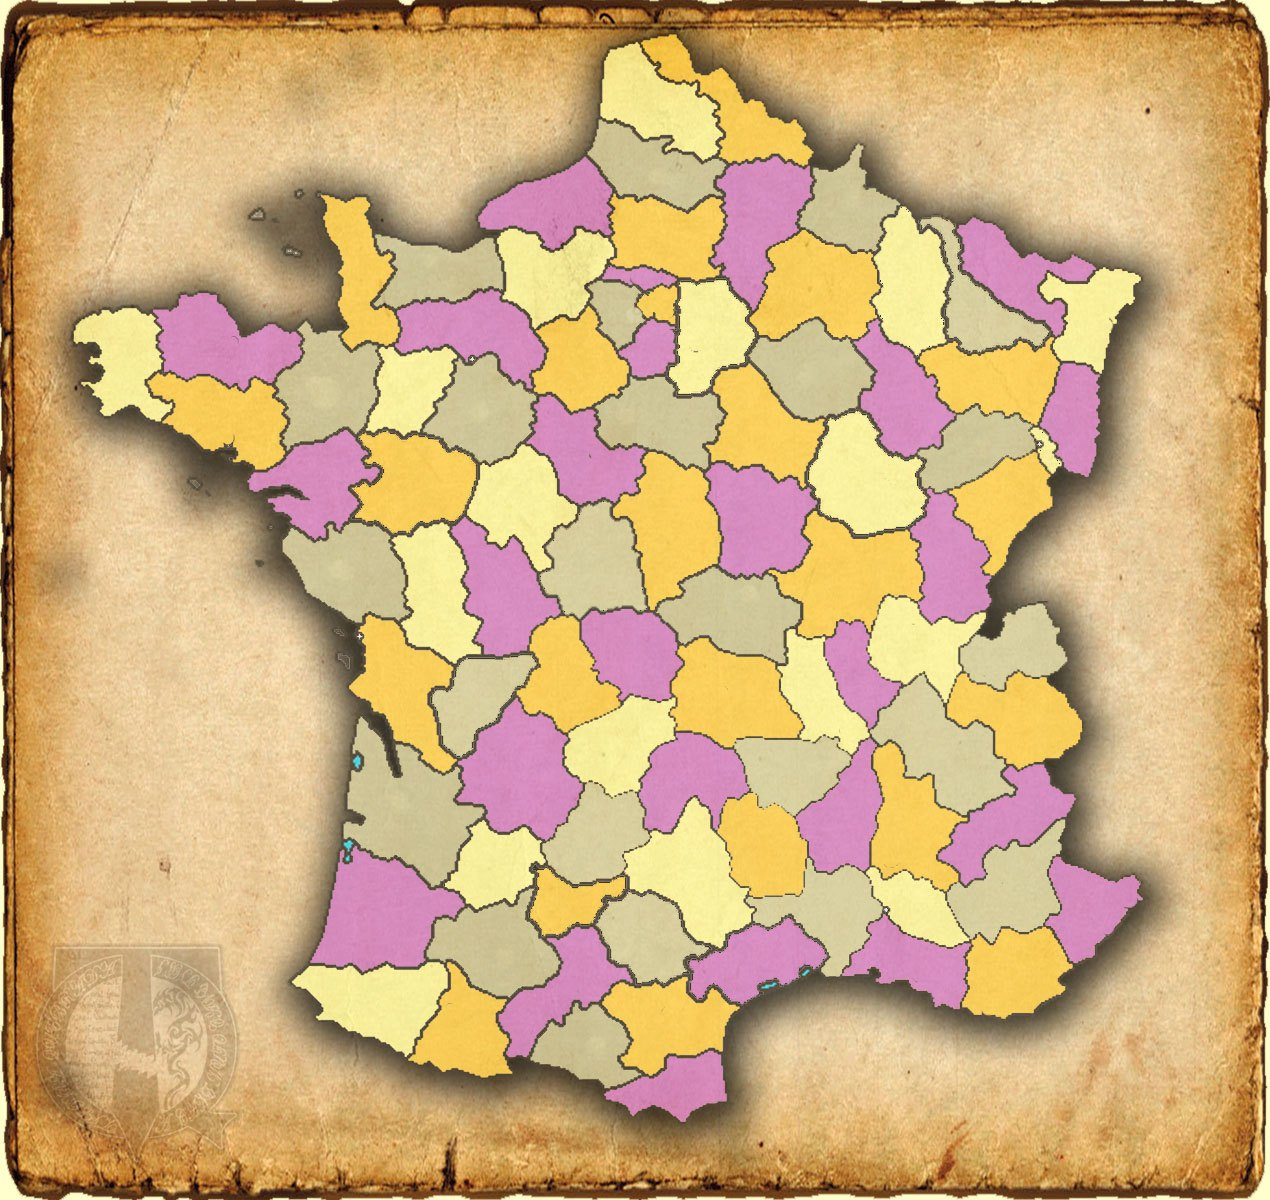
\includegraphics[width=5cm]{mapa-4-colores_HR.jpg}
    \caption{Mapa político coloreado}
\end{figure}
\end{minipage}
\begin{minipage}[c]{5cm}
\begin{block}{Mapa conexo}\em
Un mapa es conexo\footnote{de una pieza} y cada una de sus regiones también es conexa.
\end{block}
\end{minipage}
\end{frame}

\begin{frame}{\insertsection}
\begin{block}{}
Dos regiones no pueden tocarse solo en un punto, y así, se pueden ignorar regiones con una única línea frontera.
\end{block}
\begin{center}
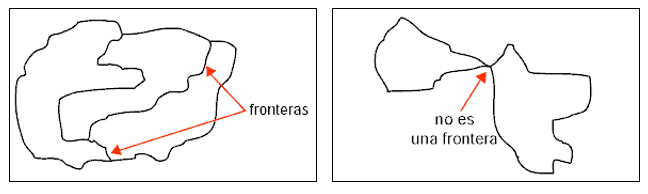
\includegraphics[height=3cm]{fronteras.png}
\end{center}

\begin{block}{}
Es un problema topológico: no importa la forma de las regiones, sino como están colocadas unas respecto a otras.
\end{block}
\end{frame}

%%%%%%%%%%%%%%%%%%%%%%%%%%%%%%%%%%%%%%%%%%%%%%%%%%%%%%%%%%%%%%%%%%%

\begin{frame}{\insertsection}\transblindsvertical
Leonhard Euler
\begin{block}{Fórmula de Euler para mapas:}
$$
\#\text{caras} - \#\text{aristas} + \#\text{vértices} = 2.
$$
\end{block}
\begin{center}
   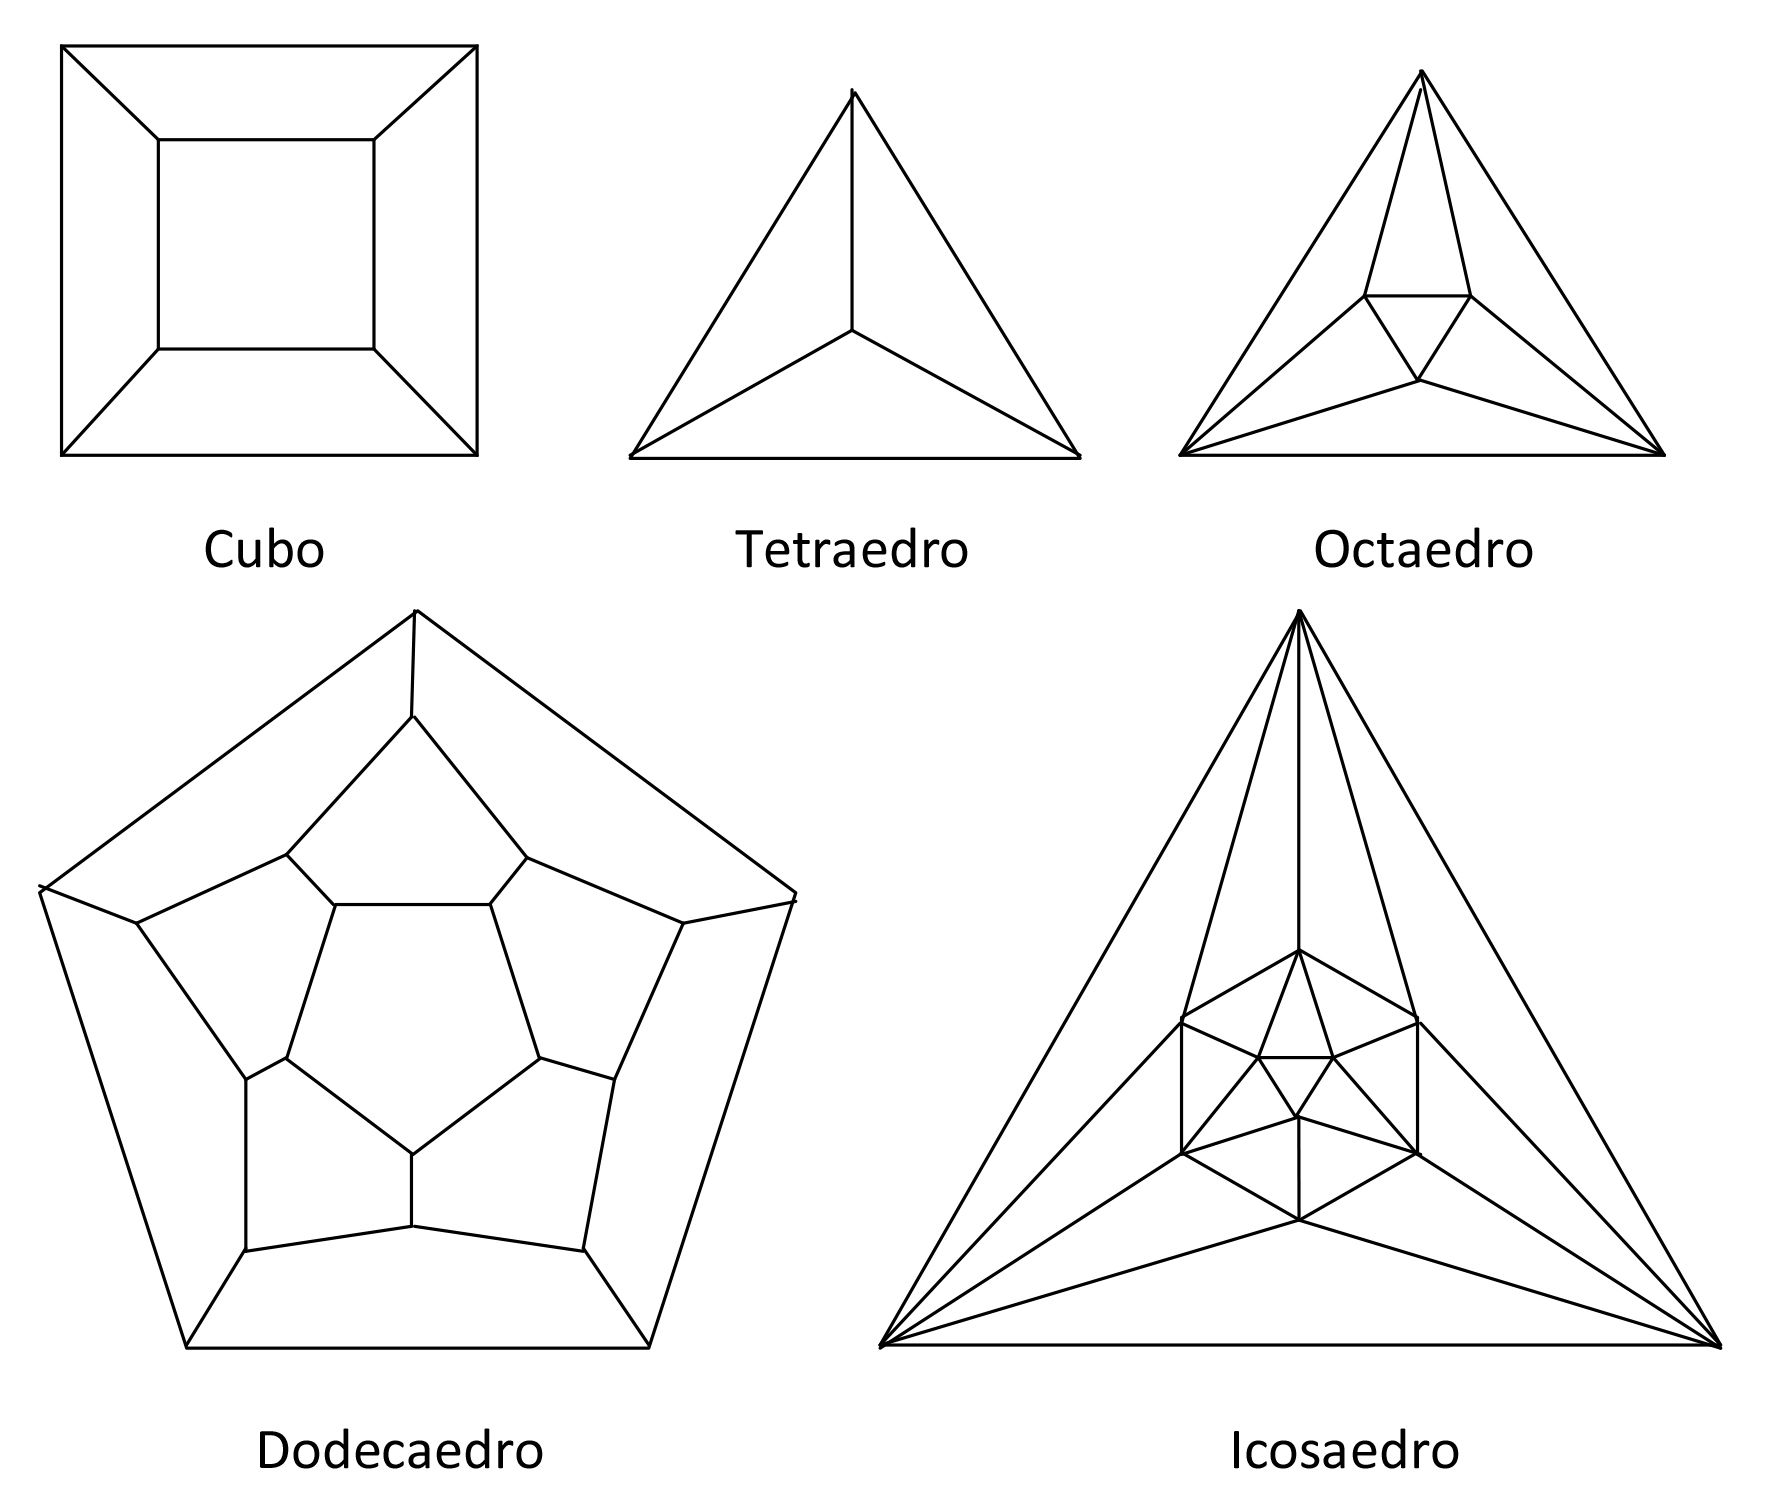
\includegraphics[height=5cm]{poliedros2.jpg}
\end{center}
\end{frame}
\section{Historia}

\begin{frame}{\insertsection}\transblindsvertical
Línea del Tiempo
\centering
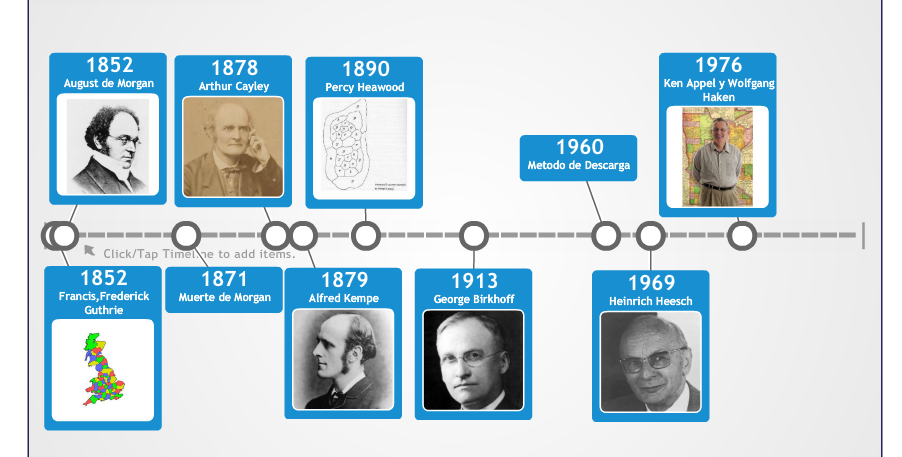
\includegraphics[width=12.5cm]{linea.png}    
\end{frame}


\begin{frame}{Personajes}
\centering
\begin{minipage}[c]{3cm}
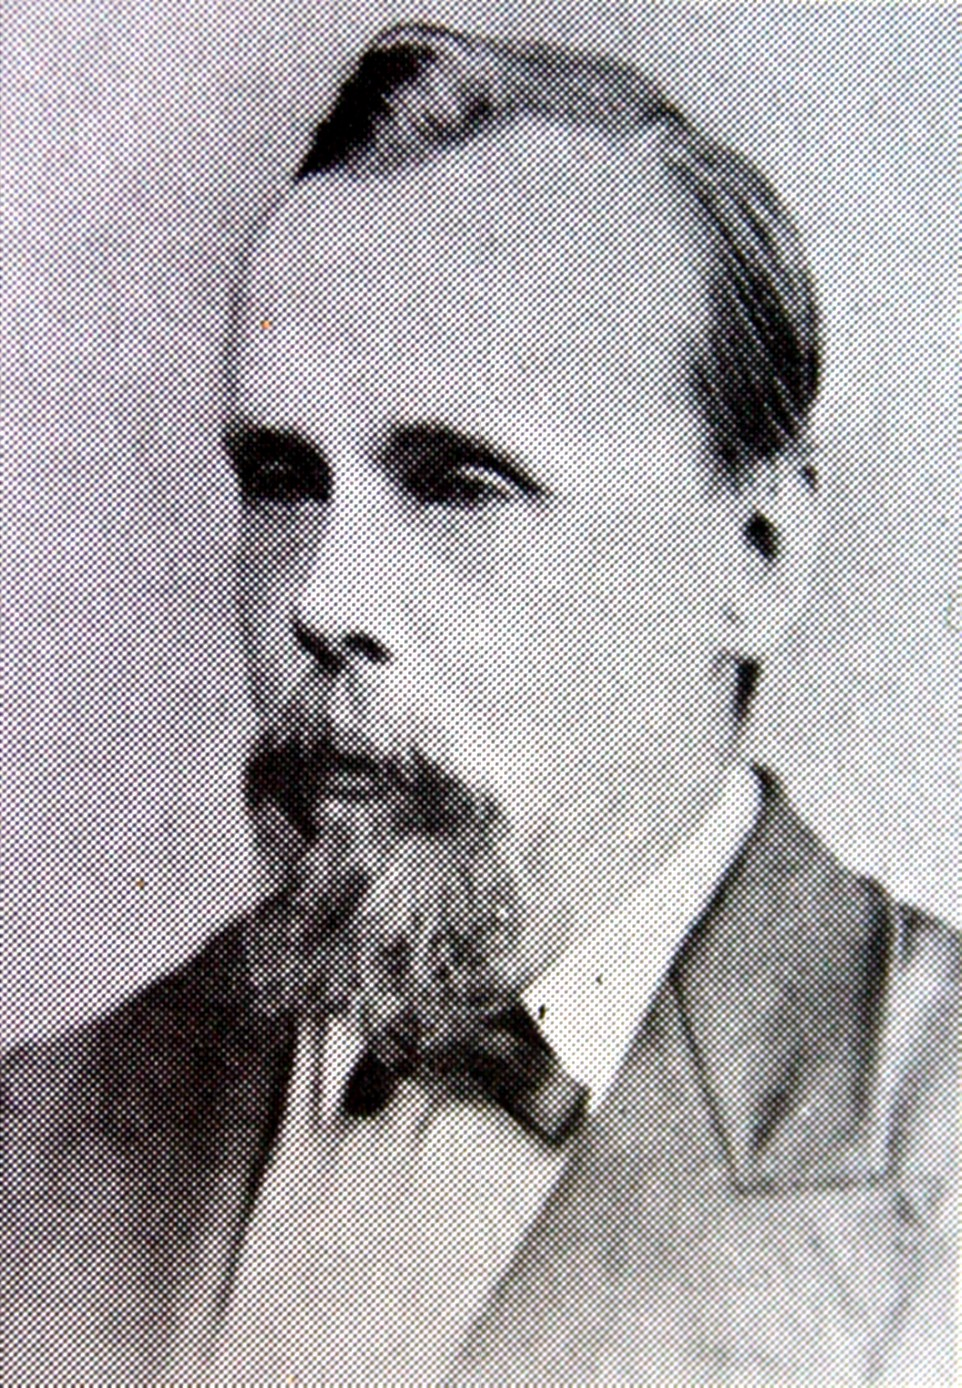
\includegraphics[width=2.5cm]{Francis_guthrie} \\
\centering \bf{FRANCIS GUTHRIE}
\end{minipage}
\begin{minipage}[c]{4cm}
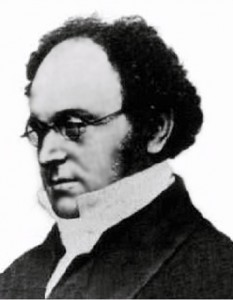
\includegraphics[width=2.5cm]{morgan.jpg}\\
\centering\bf{AUGUST DE MORGAN}
\end{minipage}
\begin{minipage}[c]{3cm}
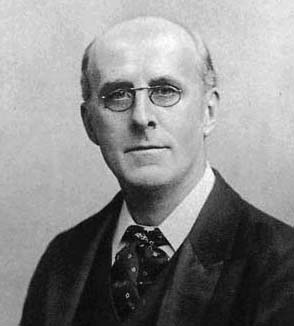
\includegraphics[width=2.5cm]{kempe.jpeg}\\
\centering\bf{ALFRED BRAY KEMPE}
\end{minipage}
\end{frame}

\begin{frame}{\insertsection}\transblindsvertical
Fechas importantes
\begin{itemize}
    \item 1852: Francis Guthrie plantea el problema a su hermano Frederick y éste a Augustus de Morgan.
    
    \item  1878: Arthur Cayley publica el enunciado de la conjetura.
    
    \item  1879: Sir Alfred Bray Kempe publica su demostración.
    
    \item  1913: George Birkhoff introduce la noción de configuración reducible.
    
    \item  1960: Se introduce el llamado método de descarga.
    
    \item  1969: Avances de Heinrich Heesch en reducibilidad y obtención de conjuntos inevitables de configuraciones.
    
    \item 1976: Ken Appel y Wolfgang Haken prueban con ayuda de un ordenador que sus 1.482 configuraciones son reducibles (50 días de cálculo).
    
    \item  1996: N. Robertson, D.P. Sanders, P. Seymour y R. Thomas mejoran la demostración con ayuda de ordenador (sólo 633 configuraciones) y automatizan la prueba de la inevitabilidad.
\end{itemize}   
\end{frame}

\begin{frame}{\insertsection}\transblindsvertical
\begin{flushright}
\begin{block}{Francis Guthrie (1839-1899)}
Abogado y botánico, observa que puede colorear un mapa complejo de los cantones de Inglaterra con 4 colores. En 1852, enuncia el problema a su hermano Frederick (University College London) y a éste a Augustus de Morgan. Francis Guthrie observa que 3 colores no son suficientes, con el diagrama crítico:
\end{block}
\begin{figure}
  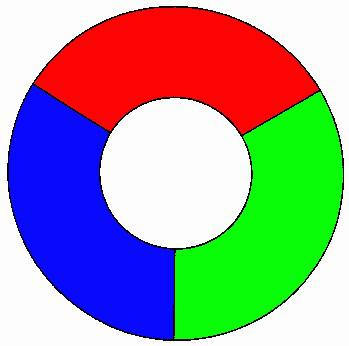
\includegraphics[scale=0.3]{diagrama.jpg}
    \caption{Diagrama Crítico}
\end{figure}
\end{flushright}
\end{frame}

\begin{frame}{\insertsection}\transblindsvertical
August de Morgan
\begin{block}{Difusión del teorema}
Augustus de Morgan (1806-1871) estaba muy interesado en la conjetura de los 4 colores y difundió entre sus colegas su importancia. Una de las primeras personas con las que ``habló'' fue con el matemático y físico irlandés Sir William Rowan Hamilton (1805-1865), que no compartía el interés de De Morgan por el problema. Le escribe una carta el 23 de octubre de 1852.
\end{block}

\begin{block}{Respuesta de Hamilton}
Cuatro días después, Hamilton le contesta: ``I am not likely to attempt your “quaternion” of colours very soon''.
\end{block}    
\end{frame}

\begin{frame}{\insertsection}\transblindsvertical
\begin{block}{Primera demostración}
Kempe se interesa por el problema de los 4 colores tras la pregunta de Cayley en la London Mathematical Society.
\end{block}

\begin{block}{}
En junio de 1879 obtiene su solución del teorema de los 4 colores y lo publica en el Amer. Journal of Maths. En 1880, publica unas versiones. simplificadas de su prueba, donde corrige algunas erratas de su prueba original, pero deja intacto el error fatal.
\end{block}
    \end{frame}

\begin{frame}{\insertsection}\transblindsvertical
El error fatal
\end{frame}

\begin{frame}{\insertsection}\transblindsvertical
Demostración definitiva
\end{frame}

\section{Aplicaciones}
\begin{frame}{\insertsection}\transblindsvertical

\end{frame}

\begin{frame}{Bibliografía}\transblindsvertical
\begin{thebibliography}{9}
	\bibitem{Kop04}
	Kopka, Helmut; Daly, Patrick W.
	\newblock {\em Guide to \LaTeX}. 4th ed.
	\newblock Pearson Education, Inc., 2004.
\end{thebibliography}
\end{frame}

\end{document}